\chapter{Dataset}
Per concludere analiziamo come il sistema si comporta sulla generazione di dataset. Si procederà in modo incrementale, per capire come affrontare lo scheduling di taskset più semplici e poi quelli più complessi.

Questa parte può essere anche utile per capire come struttrare il main ed utilizzare il simulatore.

%%%%%%%%%%%%%%%%%%%%%%%%%%%%%%%%%%%%%%%%%%%%%%%%%%%%%%%%%%%%%%%%
\section{Baseline}
Vediamo come funziona lo scheduler RM con un taskset molto semplice. Il taskset in questione, come si può notare dal codice in Figura~\ref{fig:baseline}, è molto semplice in modo da poter osservare le differenze tra le due simulazioni. Si tratta di un task con due task puramenti periodici: il primo ha periodo e deadline relativo pari a 20ms e un chunk con un exectuion time di 10ms; il secondo ha periodo e deadline di 60ms e tre chunk con execution time rispettivamente di 5ms, 4ms e 3ms.

La traccia in Figura~\ref{fig:traceBaseline} è l'output della simulazione.

\begin{figure}[htbp]
    \centering
    \begin{subfigure}{0.45\textwidth}
        \vfill
        \centering
        \raisebox{7em}{
            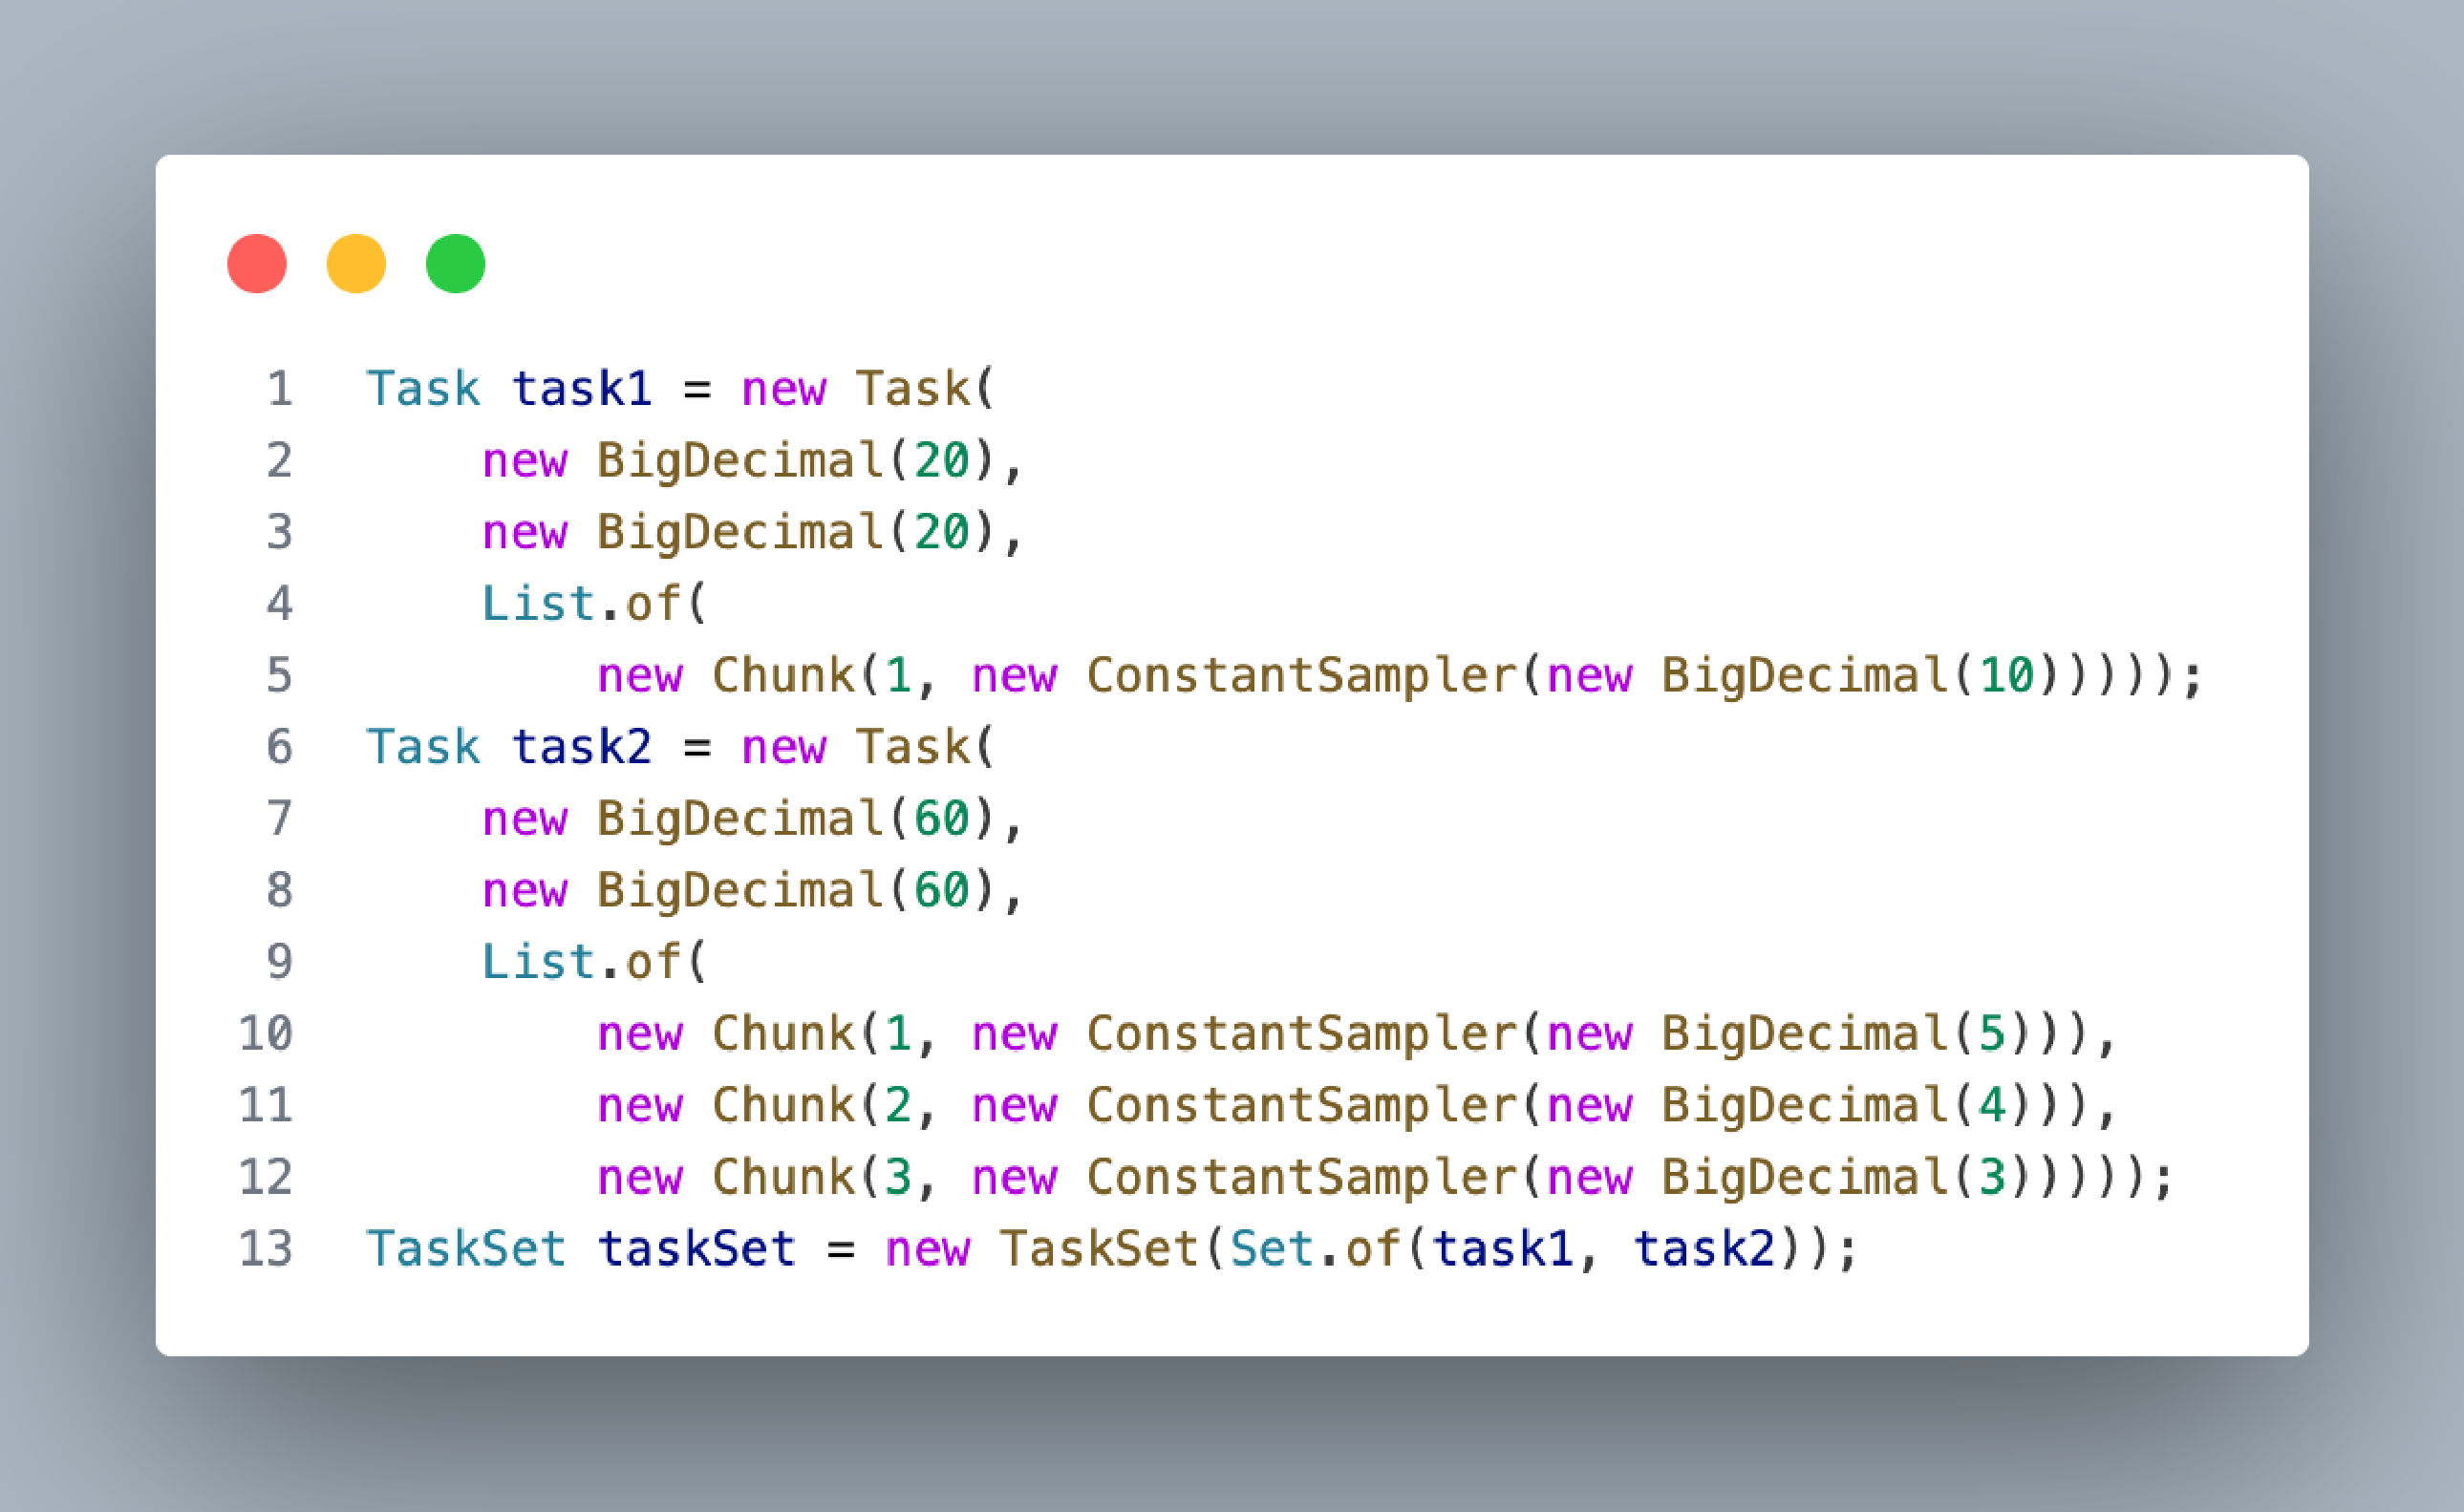
\includegraphics[width=.9\textwidth]{immagini/taskset baseline.pdf}
        }
        \caption{Taskset baseline.}
        \label{fig:baseline}
        \vfill
    \end{subfigure}
    \hfill
    \begin{subfigure}{0.45\textwidth}
        \vfill
        \centering
        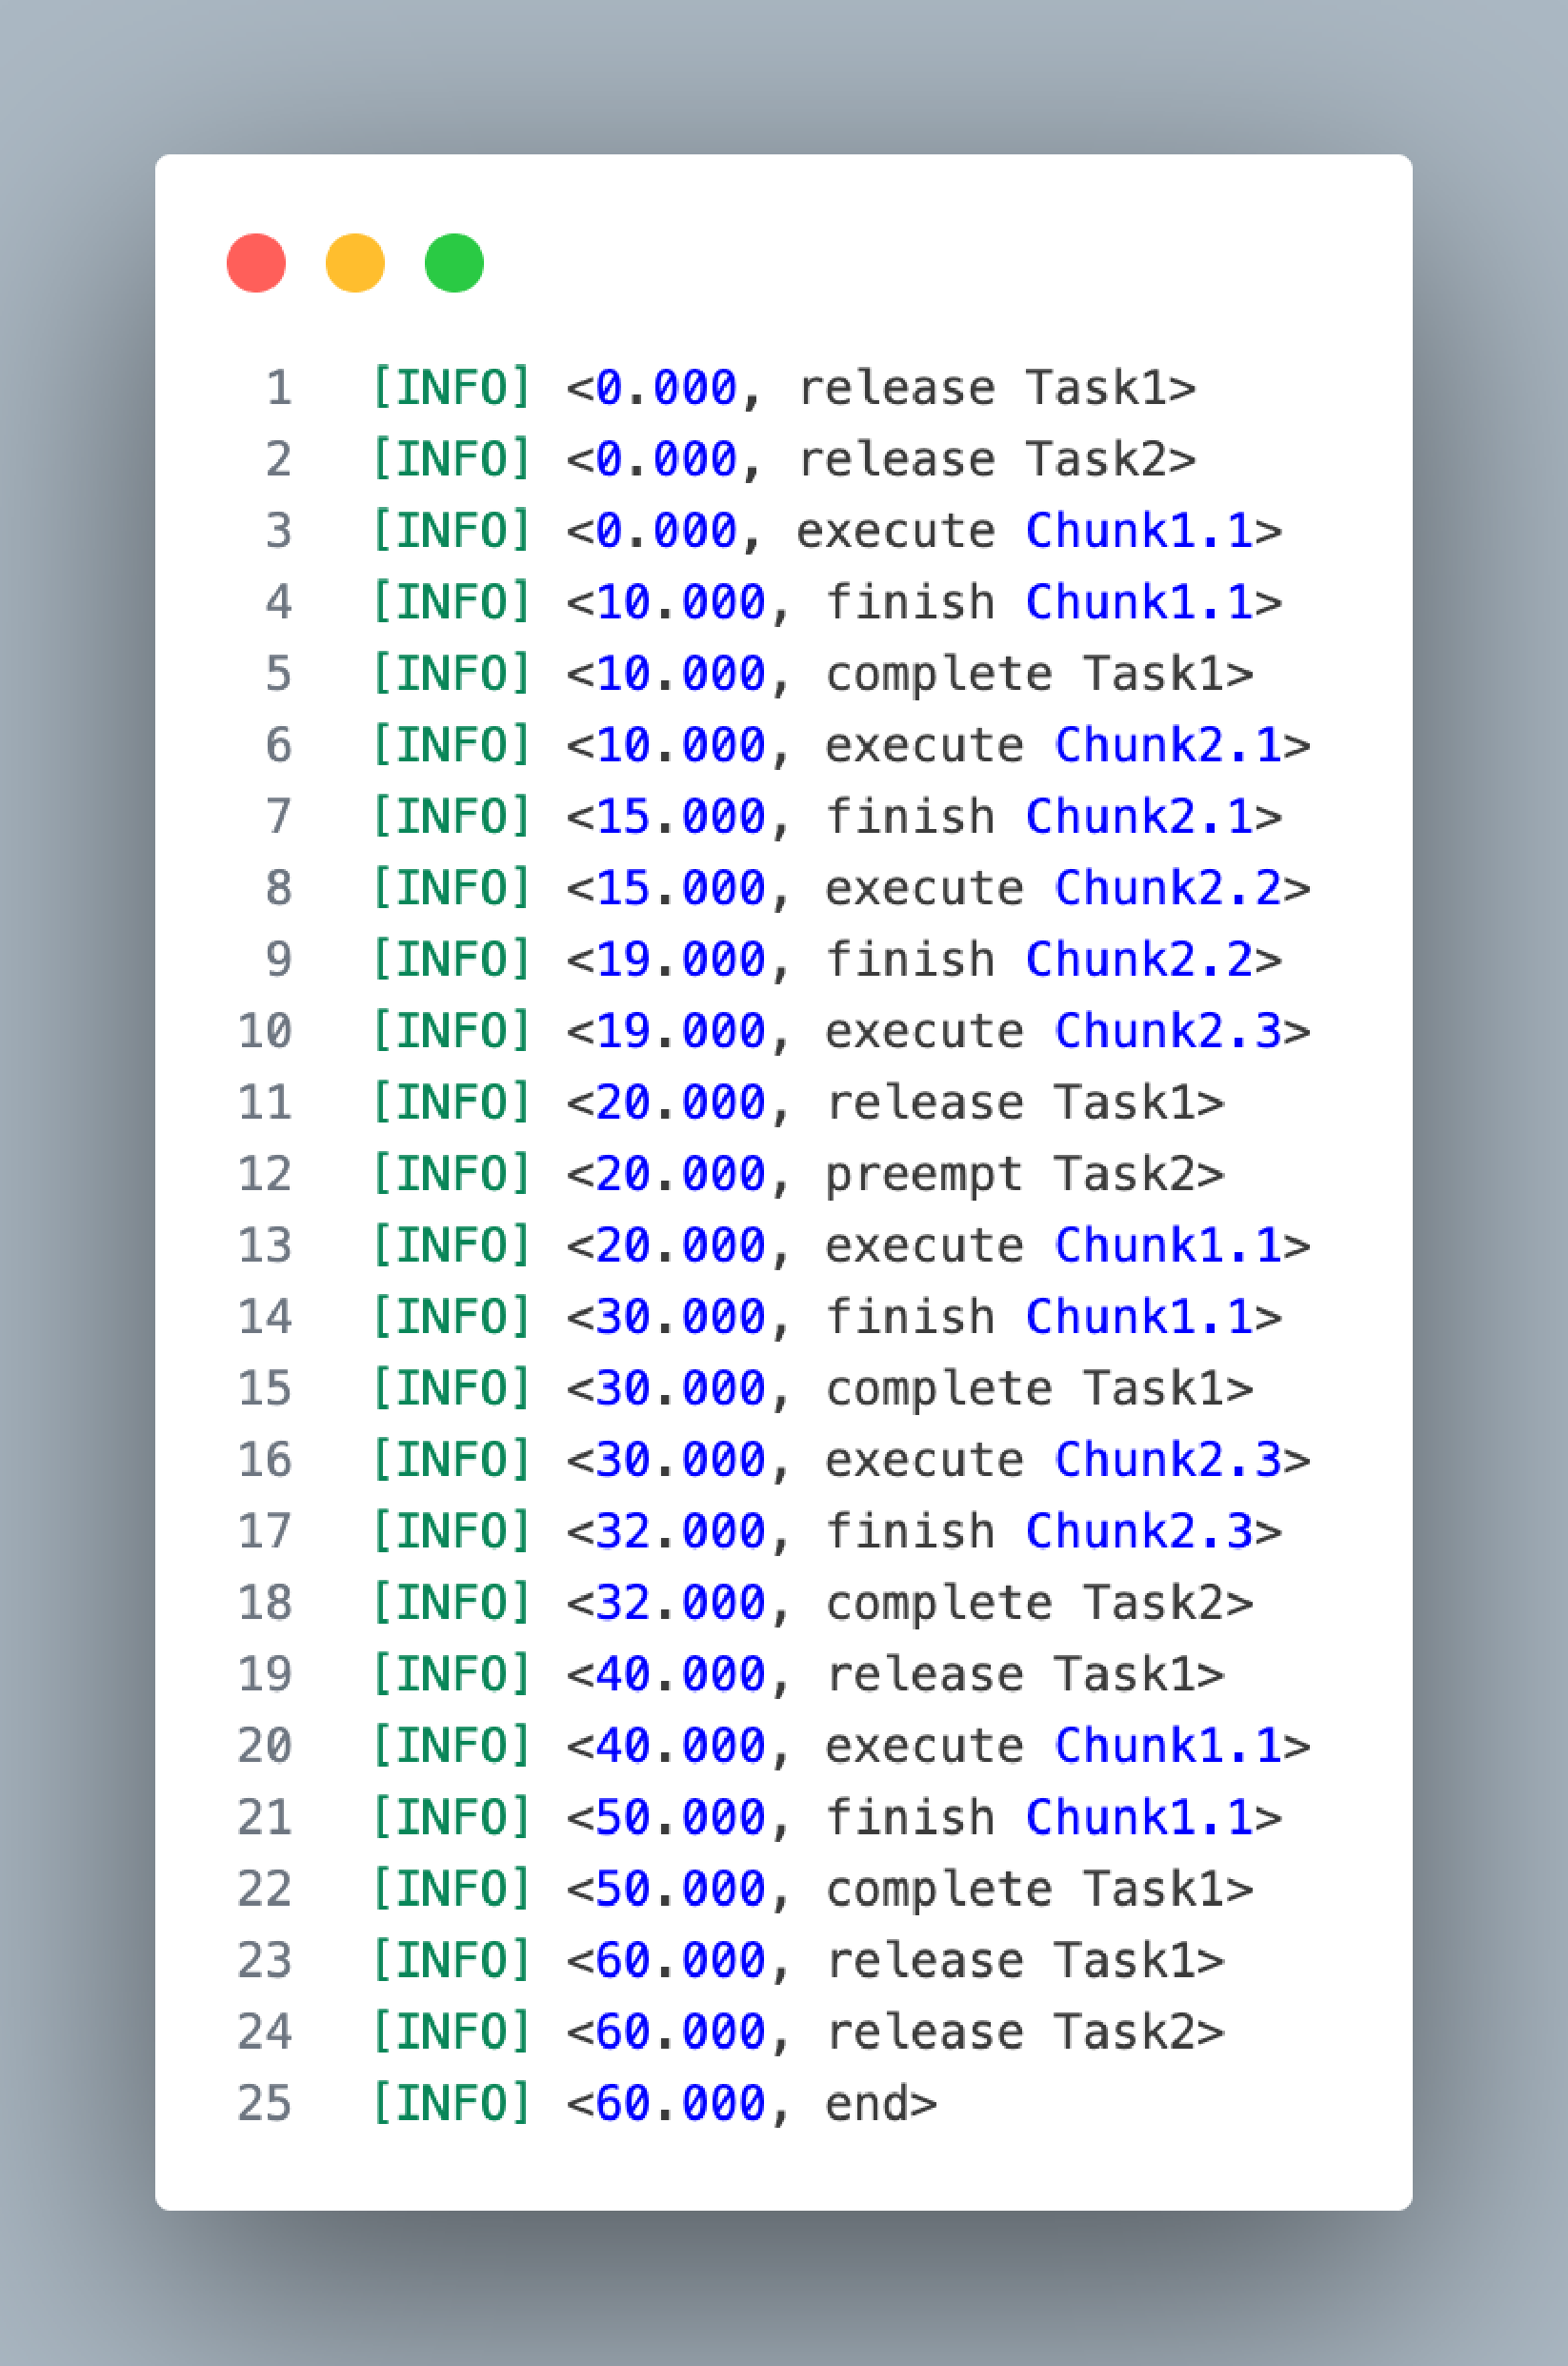
\includegraphics[width=.9\textwidth]{immagini/trace baseline.pdf}
        \caption{Traccia del task baseline.}
        \label{fig:traceBaseline}
        \vfill
    \end{subfigure}
    \caption{Baseline.}
\end{figure}